\section{Offline initial opportunity and bounded paths}
The declared initial domain contains $k(154-k)$ replacements: 600, 1168, and 2208 at $k=4,8,16$. All feasible endpoints are labeled in the 96 available cells. The 2016 late-state prerequisite exclusion leaves three unrun cells in the 99-cell denominator. Teacher labels never enter proposal, ranking, acceptance, or threshold selection.

For each complete object, we sum the positive full-dictionary best gain over its nine initial cells. Dividing the sum of anchor top-one verified/no-op gains by this denominator measures ranking capture. Dividing the sum of best gains achievable within the fixed incoming pool measures candidate coverage. Ranking capture ranges from 0.97302 to 0.99985, with median 0.99538; short-pool coverage ranges from 0.49119 to 0.95307, with median 0.72951. These are weighted one-decision opportunities, not deployed trajectory improvement fractions. The incomplete object is displayed with its observed six-cell scope and is excluded from ten-complete-object summaries.

\begin{figure}[htbp]\centering
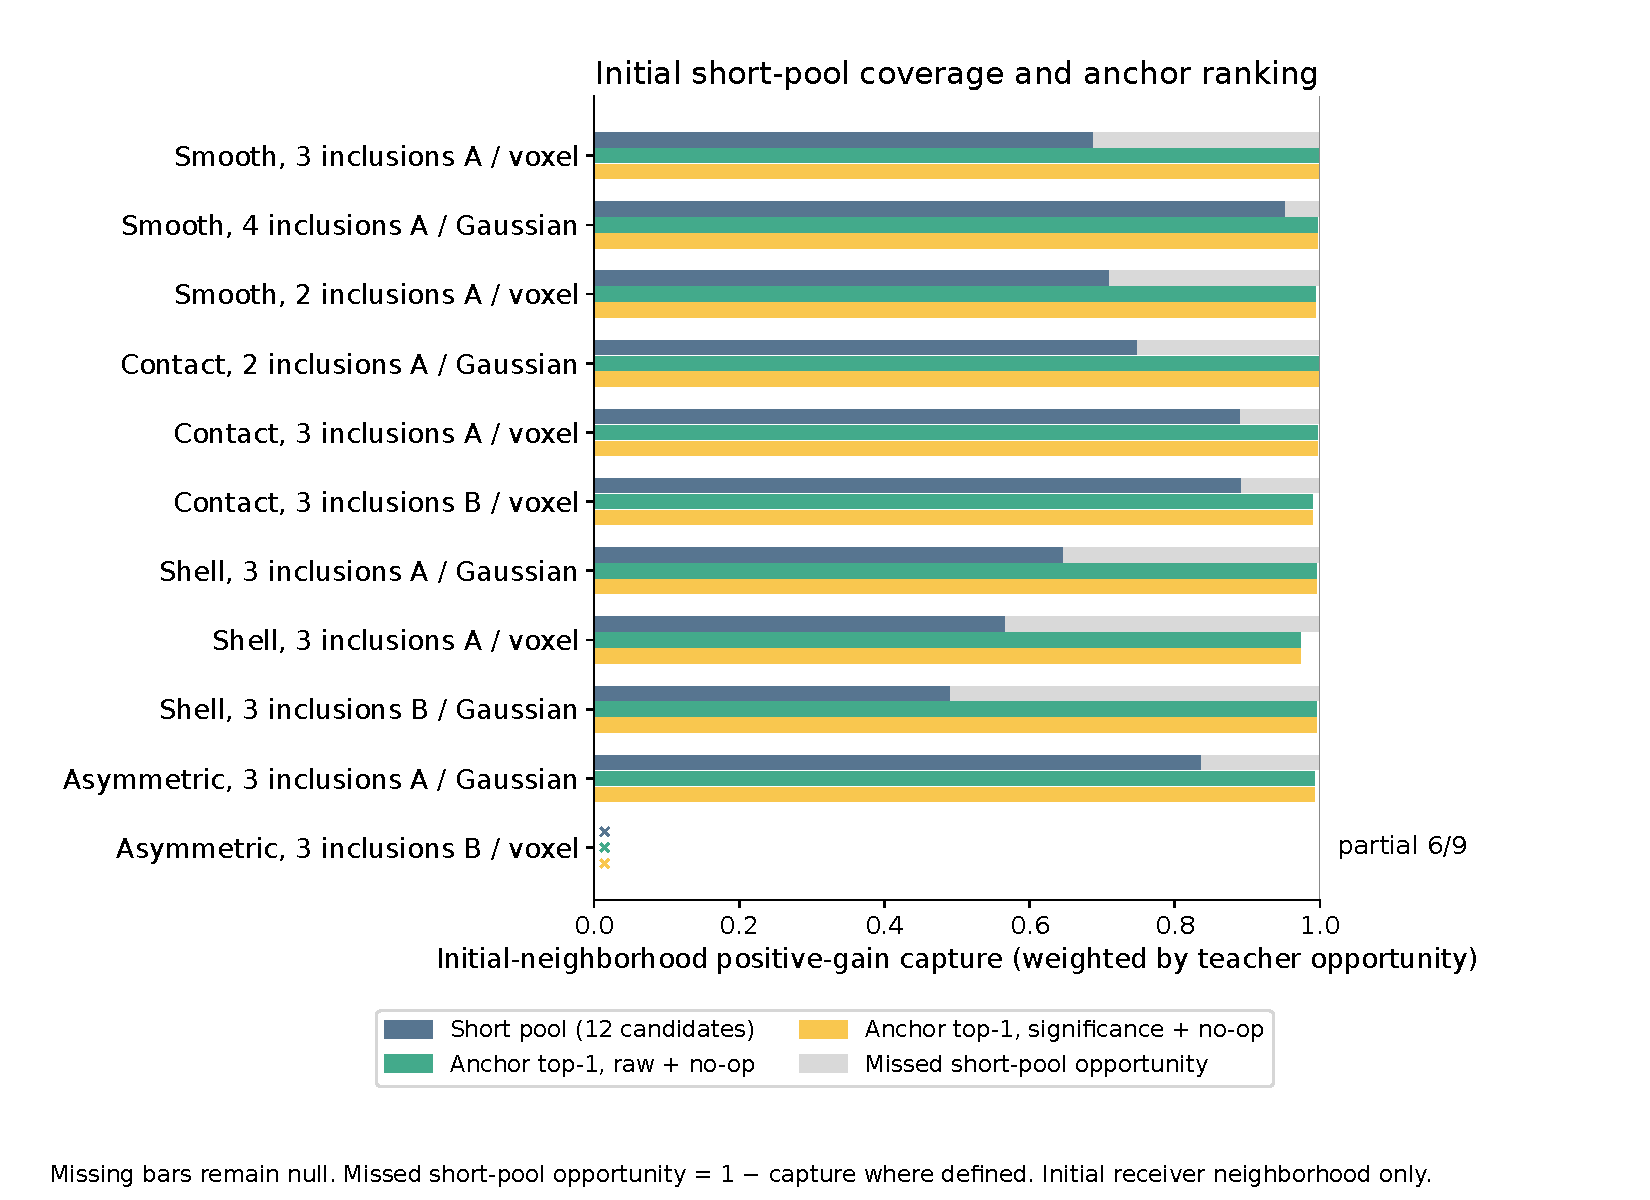
\includegraphics[width=.94\linewidth]{figures/coverage_closure_v2/initial_opportunity.pdf}
\caption{Initial receiver-neighborhood opportunity, separating reduced ranking from acquisition into the frozen 12-atom pool. Missing cells are not imputed.}
\end{figure}
\begin{figure}[htbp]\centering
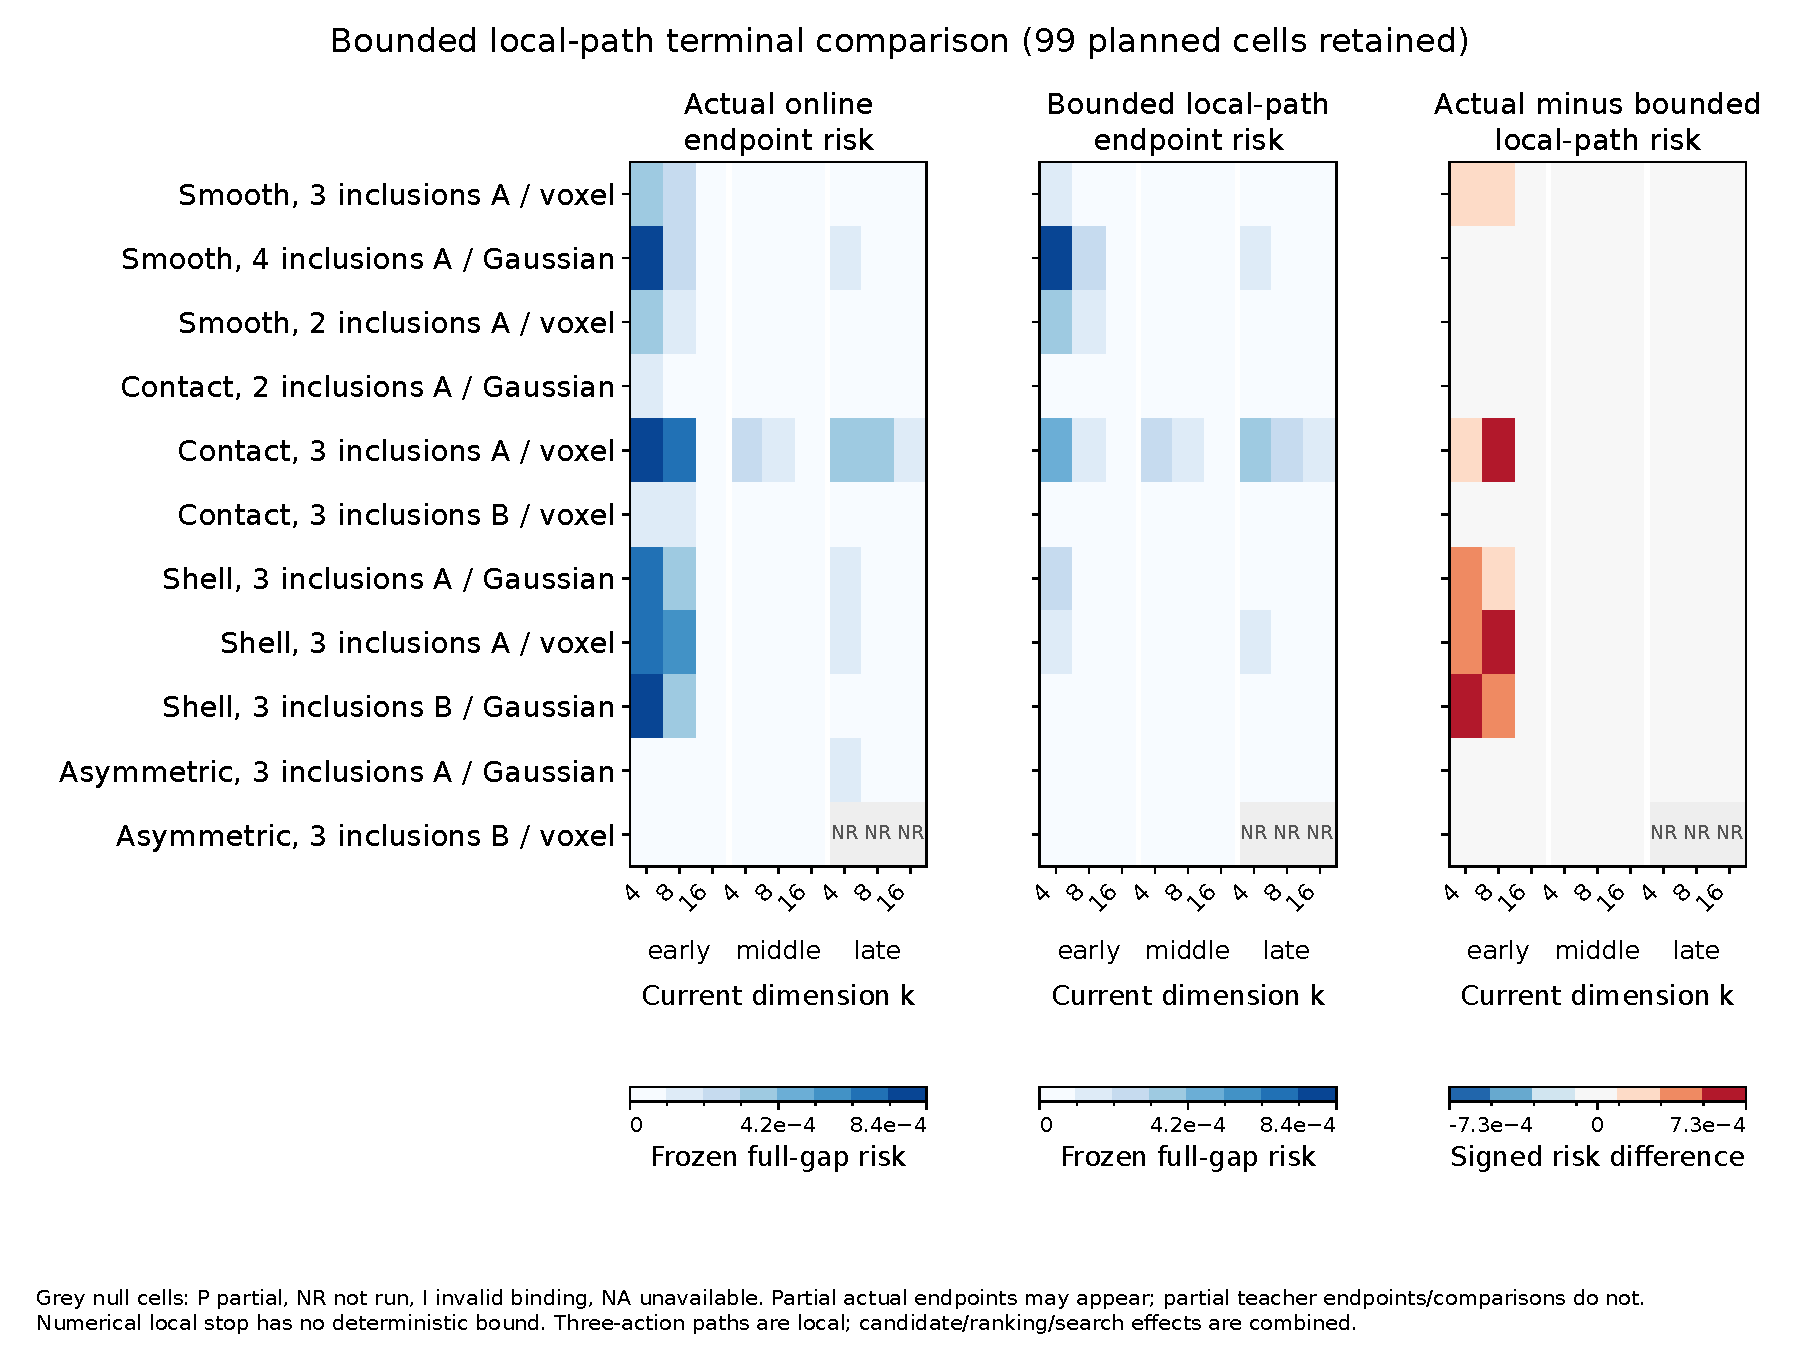
\includegraphics[width=.98\linewidth]{figures/coverage_closure_v2/bounded_path_risk.pdf}
\caption{Online and offline bounded-path final gaps. The teacher recomputes a full local one-swap neighborhood at each accepted step and stops after at most three actions. It is not a global oracle. Five online paths outperform the greedy teacher path, 90 teacher paths outperform deployment, and one differs only within the evaluation floor. These comparisons combine candidate coverage, ranking, and search interactions.}
\end{figure}
